        \documentclass{standalone}
        \usepackage{tikz}
        \usetikzlibrary{arrows}
        \usepackage{amsmath}
        \usepackage{amsfonts}
        \begin{document}
        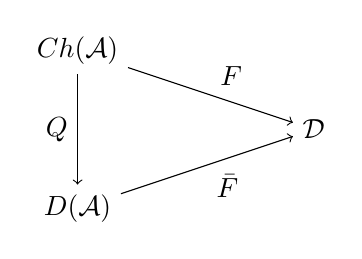
\begin{tikzpicture}

    \node (CA) at (-2,0) {$Ch(\mathcal A)$};
    \node (D) at (1,-1) {$\mathcal D$};
    \node (DA) at (-2,-2) {$D(\mathcal A)$};
    \draw[->] (CA) -- node[above right] {$F$} (D);
    \draw[->] (CA) -- node[left] {$Q$} (DA);
    \draw[->] (DA) -- node[below right] {$\bar{F}$} (D);
        \end{tikzpicture}
        \end{document}
